% !TEX TS-program = pdflatex
% !TEX encoding = UTF-8 Unicode
% !TEX root = ../main.tex
% !TEX spellcheck = en-US
% ****************************************************************************************
% File: results.tex
% Author: Jakob Spindler
% Date: 2024-10-16
% ****************************************************************************************
\chapter{Results}
\label{chapter:results}

\section{Controller Design Results}
\label{section:controller_design_results}

\begin{figure}[htbp]
    \centering
    \begin{subfigure}[b]{0.49\textwidth}
        \centering
        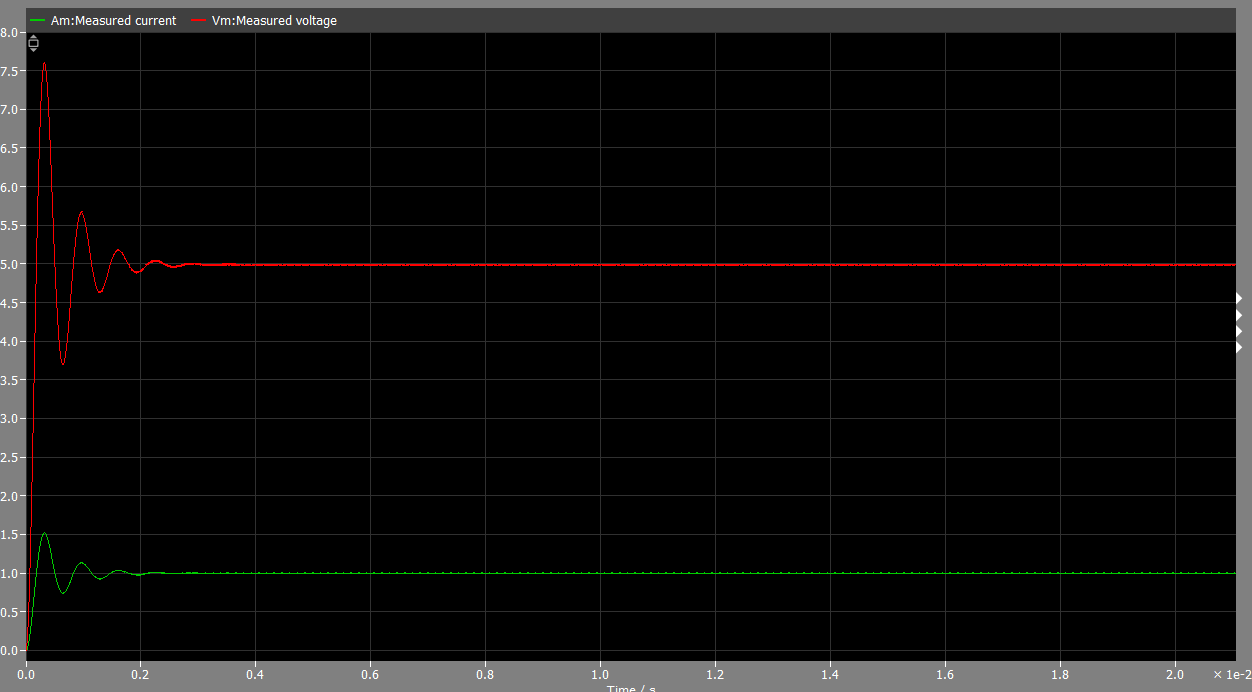
\includegraphics[width=\textwidth]{img/v_i_zoomed_constant_load.png}
        \caption{Startup behaviour of the uncontrolled converter}
        \label{fig:v_i_startup_uncontrolled}
    \end{subfigure}
    \hfill
    \begin{subfigure}[b]{0.49\textwidth}
        \centering
        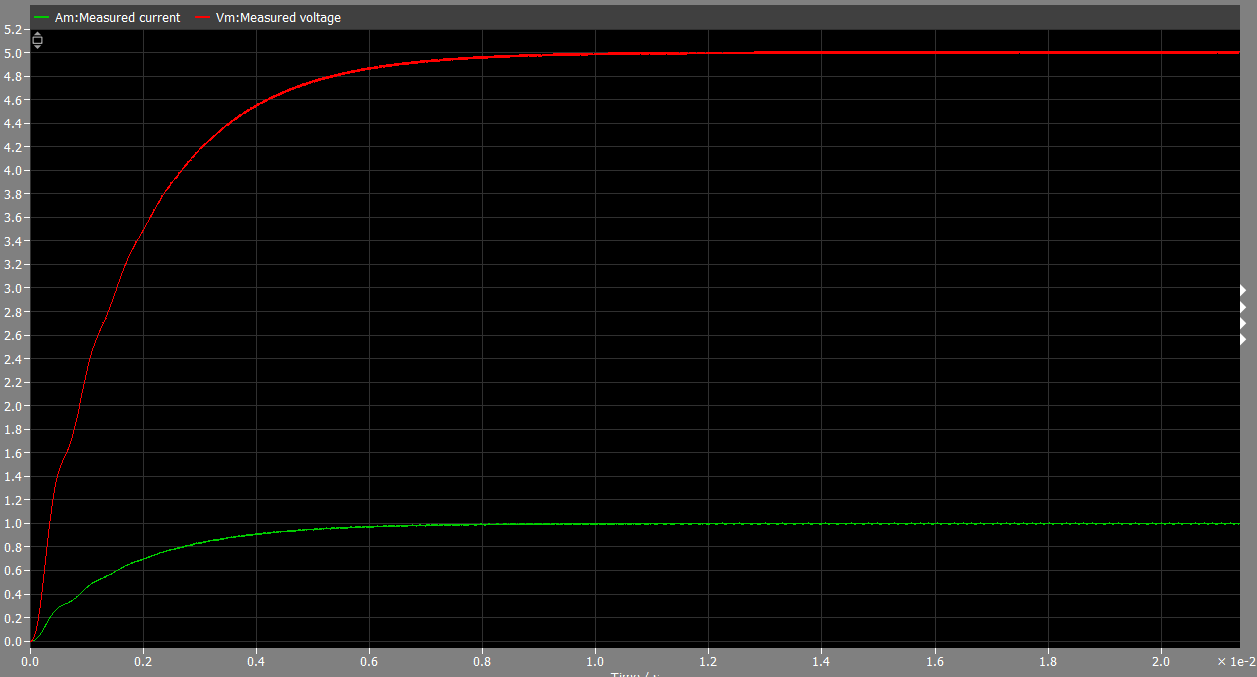
\includegraphics[width=\textwidth]{img/v_i_zoomed_control_constant_load.png}
        \caption{Startup behaviour of the controlled converter}
        \label{fig:v_i_startup_controlled}
    \end{subfigure}
    \caption{Comparison of the startup behaviour of the uncontrolled and controlled converter with current (green) and voltage (red) signals}
    \label{fig:comparison_startup}
\end{figure}

\begin{figure}[htbp]
    \centering
    \begin{subfigure}[b]{0.49\textwidth}
        \centering
        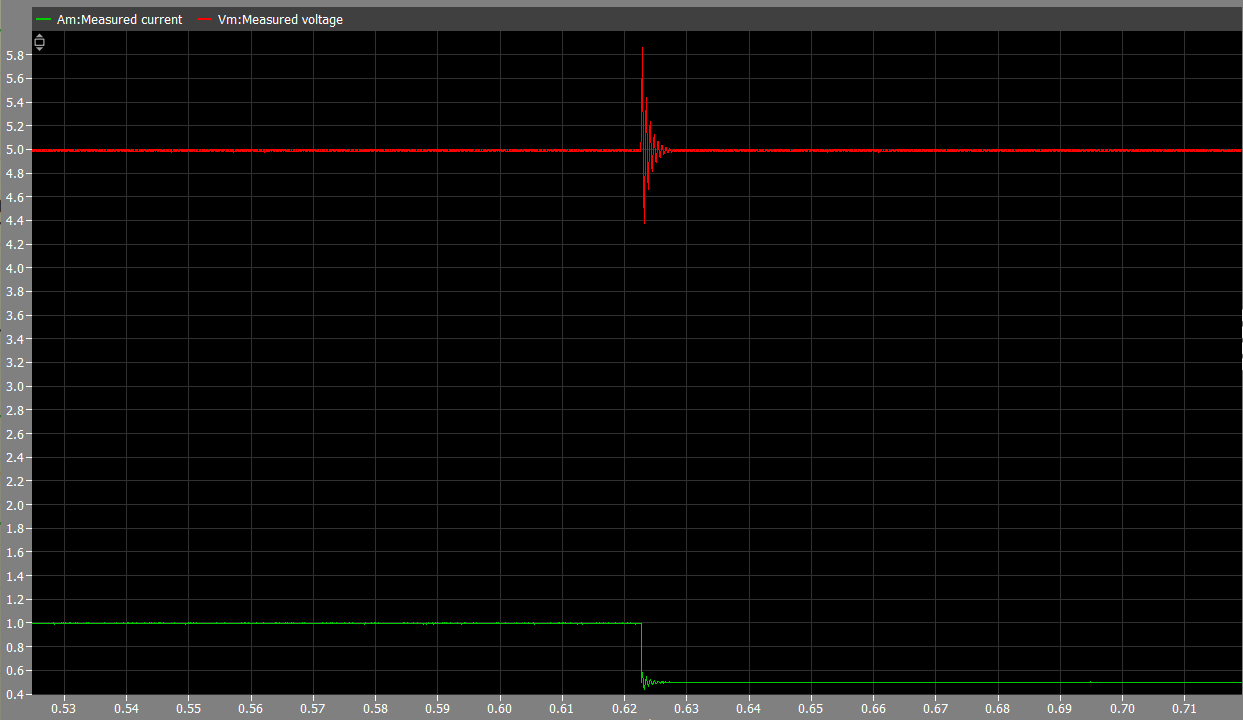
\includegraphics[width=\textwidth]{img/v_i_load_jump.png}
        \caption{load-jump behaviour of the uncontrolled converter}
        \label{fig:v_i_load_jump_uncontrolled}
    \end{subfigure}
    \hfill
    \begin{subfigure}[b]{0.49\textwidth}
        \centering
        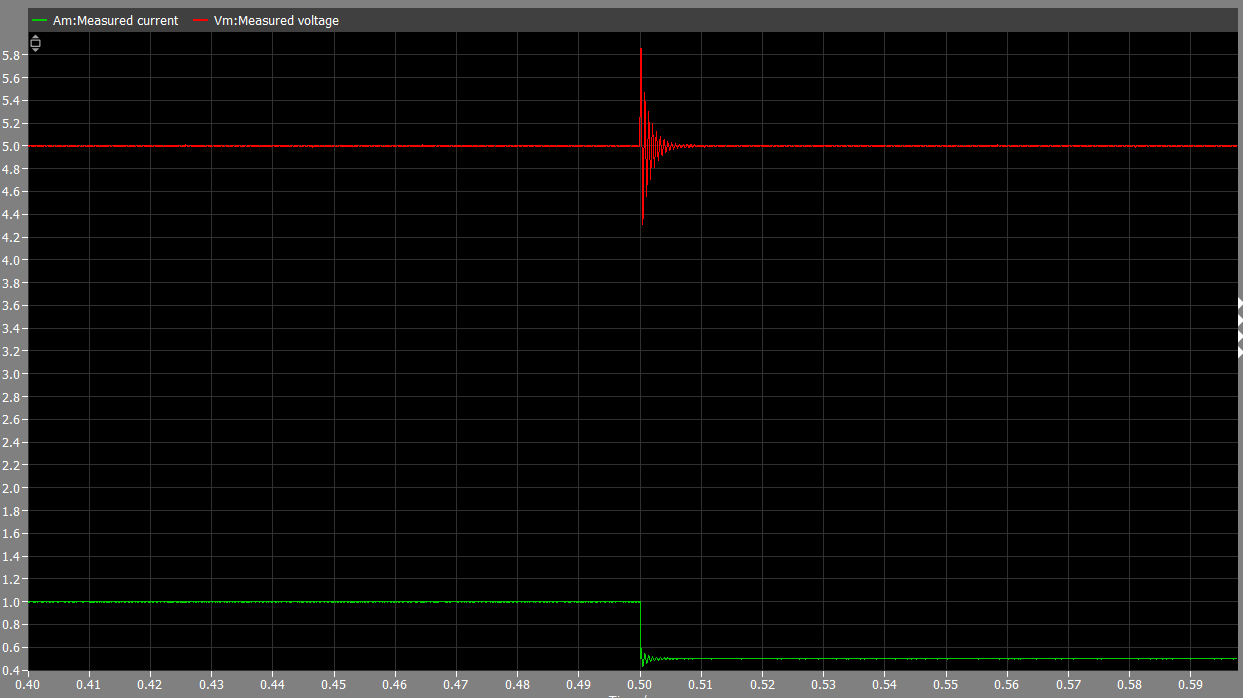
\includegraphics[width=\textwidth]{img/v_i_control_load_jump.png}
        \caption{load-jump behaviour of the controlled converter}
        \label{fig:v_i_load_jump_controlled}
    \end{subfigure}
    \caption{Comparison of the load-jump behaviour of the uncontrolled and controlled converter with current (green) and voltage (red) signals}
    \label{fig:comparison_load_jump}
\end{figure}

\begin{figure}[htbp]
    \centering
    \begin{subfigure}[b]{0.49\textwidth}
        \centering
        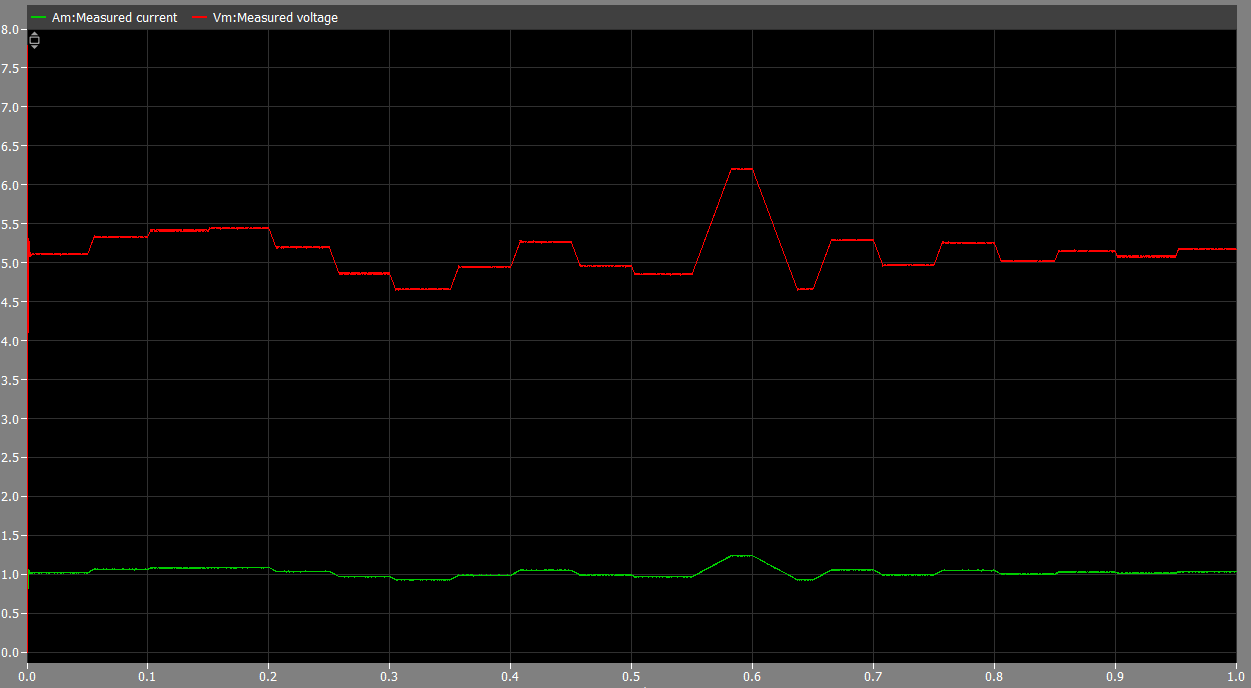
\includegraphics[width=\textwidth]{img/v_i_noise_constant_load.png}
        \caption{input noise feedthrough of the uncontrolled converter}
        \label{fig:v_i_noise_feedthrough_uncontrolled}
    \end{subfigure}
    \hfill
    \begin{subfigure}[b]{0.49\textwidth}
        \centering
        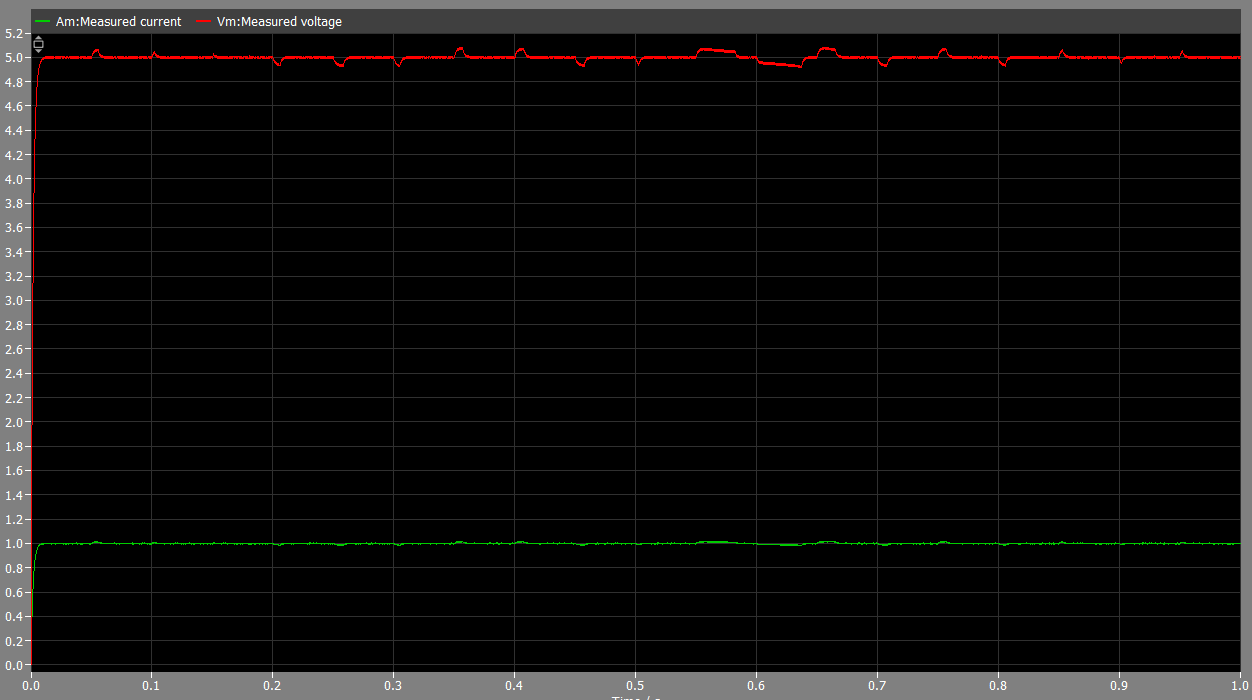
\includegraphics[width=\textwidth]{img/v_i_noise_control_constant_load.png}
        \caption{input noise feedthrough of the controlled converter}
        \label{fig:v_i_noise_feedthrough_controlled}
    \end{subfigure}
    \caption{Comparison of the input noise feedthrough behaviour of the uncontrolled and controlled converter with current (green) and voltage (red) signals}
    \label{fig:comparison_input_noise_feedthrough}
\end{figure}

\section{HIL Results}
\label{section:hil_results}

\begin{figure}[htbp]
    \centering
    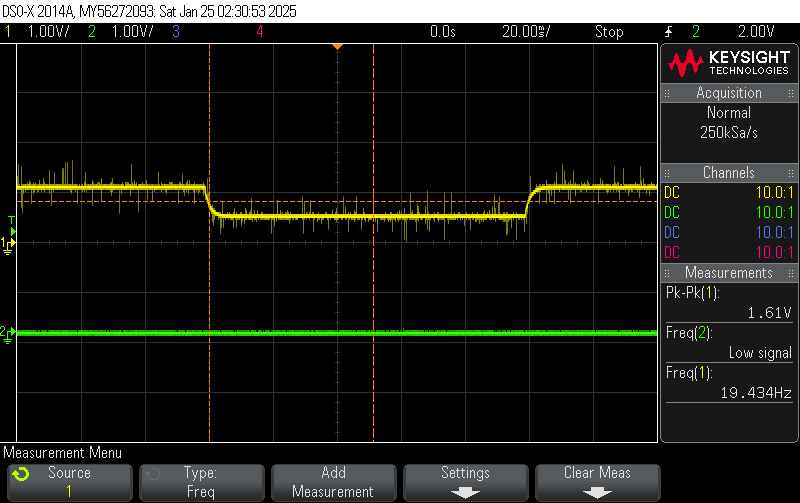
\includegraphics[width= 0.8\textwidth]{scope/scope_0.png}
    \caption{$V_{out}/5$ (ch1 - yellow) and PWM signal (ch2 - green) with vout }
    \label{fig:scope_output}
\end{figure}

\begin{figure}[htbp]
    \centering
    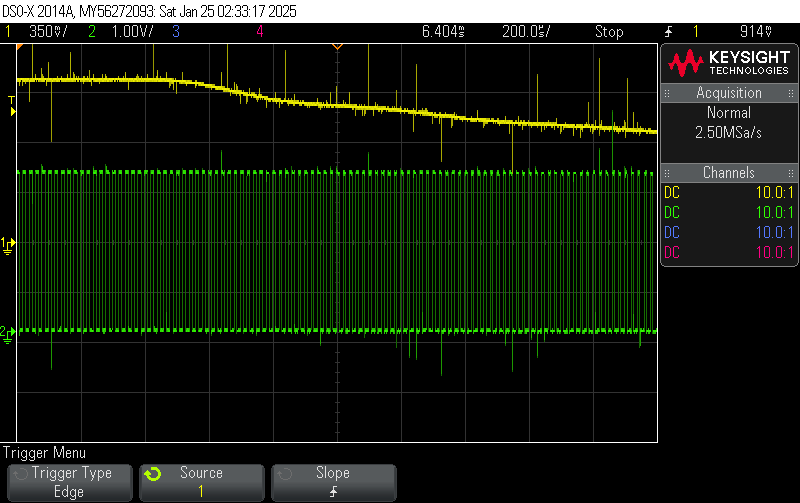
\includegraphics[width= 0.8\textwidth]{scope/scope_1.png}
    \caption{Scope output of the HIL simulation}
    \label{fig:scope_output}
\end{figure}



% EOF